\section{Anforderungen an die Jexam-Testsuite}

Wie bereits in der Einleitung erwähnt, läuft die \Gls{jexam_2009}-Plattform
derzeit ohne automatische Tests. Es besteht ein dringender Bedarf, eine
Infrastruktur zum Testen der Plattform aufzubauen. Nicht nur die
grundlegenden Funktionen der Anwendung müssen getestet werden, sondern auch
die Performance und die Sicherheit. \Gls{jexam_new}, das sich in der Entwicklung
befindet, muss jedoch am Ende des Entwicklungszyklus gleich getestet werden.
Die zwei Plattformen werden mit unterschiedlichen Technologien entwickelt
und können daher nicht einheitlich getestet werden (mit Unit-Tests). Für
die Entwicklung der Testinfrastruktur wird die Blackbox-Methode verwendet.
Das bedeutet, dass die Technologien,die für die Entwicklung des alten und neuen Jexam verwendet wurden,
keine Rolle spielen beim Testen (siehe \autoref{ch:grundlagen}).
Die Frage ist , ob die Tests für die neue Plattform neu geschrieben werden
müssen, sobald sie verfügbar ist.

\subsection{JExam UI-Tests}\label{subsec:jexam-ui-tests}

Diese Methode erm\"oglicht es, eine Plattform sowie ihre Funktionen anhand
ihrer grafischen Benutzeroberfl\"ache (\acs{ui} oder \Gls{frontend}) zu
testen. Mit Hilfe moderner Werkzeuge und Frameworks ist es m\"oglich, die
Kontrolle \"uber einen Webbrowser vollautomatisch zu \"ubernehmen. Dies
erm\"oglicht es, das Verhalten eines Benutzers auf einer Weboberfl\"ache zu
simulieren. Es wurde jedoch bereits erw\"ahnt, dass \Gls{jexam_2009} und \Gls{jexam_new}
die gleiche grafische Benutzeroberfl\"ache haben. Es gibt jedoch einige
bemerkenswerte Unterschiede im Frontend-Code der beiden Plattformen,
die bei der Entwicklung von Tests Probleme verursachen k\"onnten
(siehe \Cref{fig:old_new}). Trotzdem gibt es eine
M\"oglichkeit, die Tests nur einmal und f\"ur alle zwei
Plattformen zu schreiben. Auf diese Weise sparen die Tester Zeit und k\"onnen
herausfinden, ob \Gls{jexam_new} genauso gut funktioniert wie sein Vorg\"anger. Zu den Funktionen, die getestet werden müssen, gehören :
\begin{enumerate}
    \item Login
    \item Registrierung
    \item Abruf der Noten in der Übersicht und als pdf
    \item Einschreibung in Prüfungen
    \item Einschreibung in Lehrveranstaltungen
    \item Einschreibung in Seminargruppen
\end{enumerate}

\noindent
\begin{figure}
    \centering
    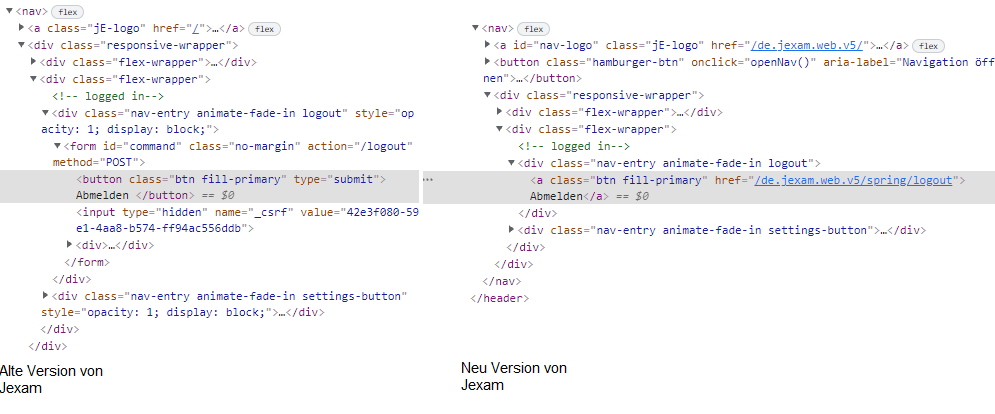
\includegraphics[scale=0.6]{images/jexam_compare}
    \caption{Frontend Quelltext von Jexam\_2009 und Jexam\_new} \label{fig:old_new}
\end{figure}


\subsection{Jexam Sicherheitstests}

Keine Software ist frei von Fehlern und Bugs. Dennoch muss eine qualitativ
hochwertige Anwendung ihren Nutzern Datenschutz garantieren. Das gilt
auch f\"ur Jexam. Das Sicherheits- oder Penetrationstesten  ist eine schwierige
Aufgabe. Das Penetrationstesten ist eine haupts\"achlich manuelle Aktivit\"at.

Experten-Penetrationtester sind ein wesentlicher Bestandteil
von Penetrationtests. Zunächst verwenden sie Schwachstellenscanner.
Es handelt sich um automatisierte Tools , die eine Umgebung untersuchen
und nach Abschluss der Untersuchung einen Bericht über die
gefundenen Schwachstellen erstellen. Diese Scanner listen diese
Schwachstellen häufig mithilfe von \Gls{cve} auf, die Informationen
über bekannte Schwachstellen liefern. Da Scanner Tausende von
Schwachstellen entdecken können, kann es sein, dass es
genügend schwerwiegende Schwachstellen gibt, die eine zusätzliche
Priorisierung erforderlich machen.


Für komplexe Tests, bei denen tief in verschiedene Systeme und
Anwendungen eingedrungen werden muss oder Übungen mit mehreren
Angriffsketten durchgeführt werden müssen, wird immer eine
erfahrenere Person oder ein erfahrenes Team benötigt. Um ein
realistisches Angriffsszenario zu testen, ist ein Team erforderlich,
das ausgeklügelte Strategien und Lösungen verwendet, die den
Techniken der Bedrohungsakteure ähneln.


Aufgrund des Ressourcenmangels im Jexam-Team muss den Prozess
automatisiert werden.  Daher sollte die Sicherheit nur
oberflächlich mit einem Schwachstellen-Scanner getestet werden.
Auf diese Weise ist es möglich hohe Vulnerabilitäten
herauszufinden, wenn sie vorhanden sind. Schwachstellen-Scans
können also auch beim Vergleich der beiden Versionen von jexam
helfen. Es wird erfahren, ob die neue Version mehr oder weniger
Schwachstellen hat als die alte. Dadurch können mögliche
Sicherheitslücken behoben werden.
\subsection{Jexam Performancestests}

\begin{center}
`` 2 Sekunden ist die Schwelle f\"ur die Akzeptanz einer E-Commerce-Website.
Bei Google streben wir eine Zeit unter einer halben Sekunde an.'' Maile Ohye
\end{center}
\>

Das obige Zitat stammt aus einem Video, das 2010 von Google Webmasters
ver\"offentlicht wurde (vgl. \cite{Ohye2010}). Wenn eine Seite l\"anger
als 2 Sekunden zum Laden braucht, verliert sie Pl\"atze in ihrer Google
\acs{seo}-Position. Es sollte sichergestellt werden, dass eine
Webanwendung dieses Kriterium erfüllt, daher ist es wichtig,
die Leistung zu testen. Die Performance einer Webanwendung spielt eine
entscheidende Rolle f\"ur die Benutzererfahrung. Jexam hat Dienste,
die immer in Echtzeit verf\"ugbar sein m\"ussen. Mithilfe von 
Performancetests kann die Anwendung unter bestimmten Bedingungen 
getestet werden, um sie zu bewerten.

Die einzelnen Schritte des Leistungstests sind von Unternehmen
zu Unternehmen und von Anwendung zu Anwendung unterschiedlich.
Sie hängen davon ab, welche Leistungsindikatoren das Unternehmen für
besonders wichtig hält. Die allgemeinen Ziele von Leistungstests
sind jedoch weitgehend identisch, so dass es einen bestimmten
Arbeitsablauf gibt, dem die meisten Testpläne folgen. Daher ist es
wichtig, die Einschränkungen, Ziele und Schwellenwerte festzulegen,
die den Erfolg des Tests belegen. Die wichtigsten Kriterien,
die für die Tests von Jexam verwendet werden, sind:

\noindent
\begin{enumerate}
    \item Die Seiten von Jexam müssen in weniger als 3 Sekunden laden,
    wenn 100 Benutzer gleichzeitig eine Anfrage stellen.
    \item Die Anwendung darf nicht spucken, wenn 2000 Nutzer
    gleichzeitig eine Seite anfordern.
\end{enumerate}

Die beiden Versionen sollten daher getestet und verglichen werden,
um eine mögliche Leistungssteigerung zu untersuchen.
Dies wird es auch ermöglichen, nach einer Änderung zu beobachten, ob
es einen Leistungsrückgang gegeben oder zum Bottlenecks geführt hat.
\subsection{Zusatzanforderungen}

Um das Schreiben und die Pflege von Tests so wenig aufwendig wie m\"oglich
zu machen, m\"ussen diese Tests au{\ss}erdem folgende Anforderungen erf\"ullen :


\textbf{Vollautomatisierung:}  Die Tests sollten vollst\"andig automatisiert sein,
um die Iteration von sich wiederholenden Aufgaben zu erm\"oglichen
und Zeit zu sparen.

\textbf{Wiederverwendung der Testsuite:} Die Testsuite muss f\"ur beide Versionen 
von jExam verwendbar sein.

\textbf{Hohe Wartbarkeit:} Die Testinfrastruktur und das Schreiben der Tests
m\"ussen leicht zu warten und einfach zu verwenden sein.

\textbf{Leicht zu installieren:} Die Testinfrastruktur muss einfach zu installieren sein und muss
unter Windows, MAC und Linux laufen k\"onnen.

